\subsection{Figures}
\begin{figure}[!htb]
\centering
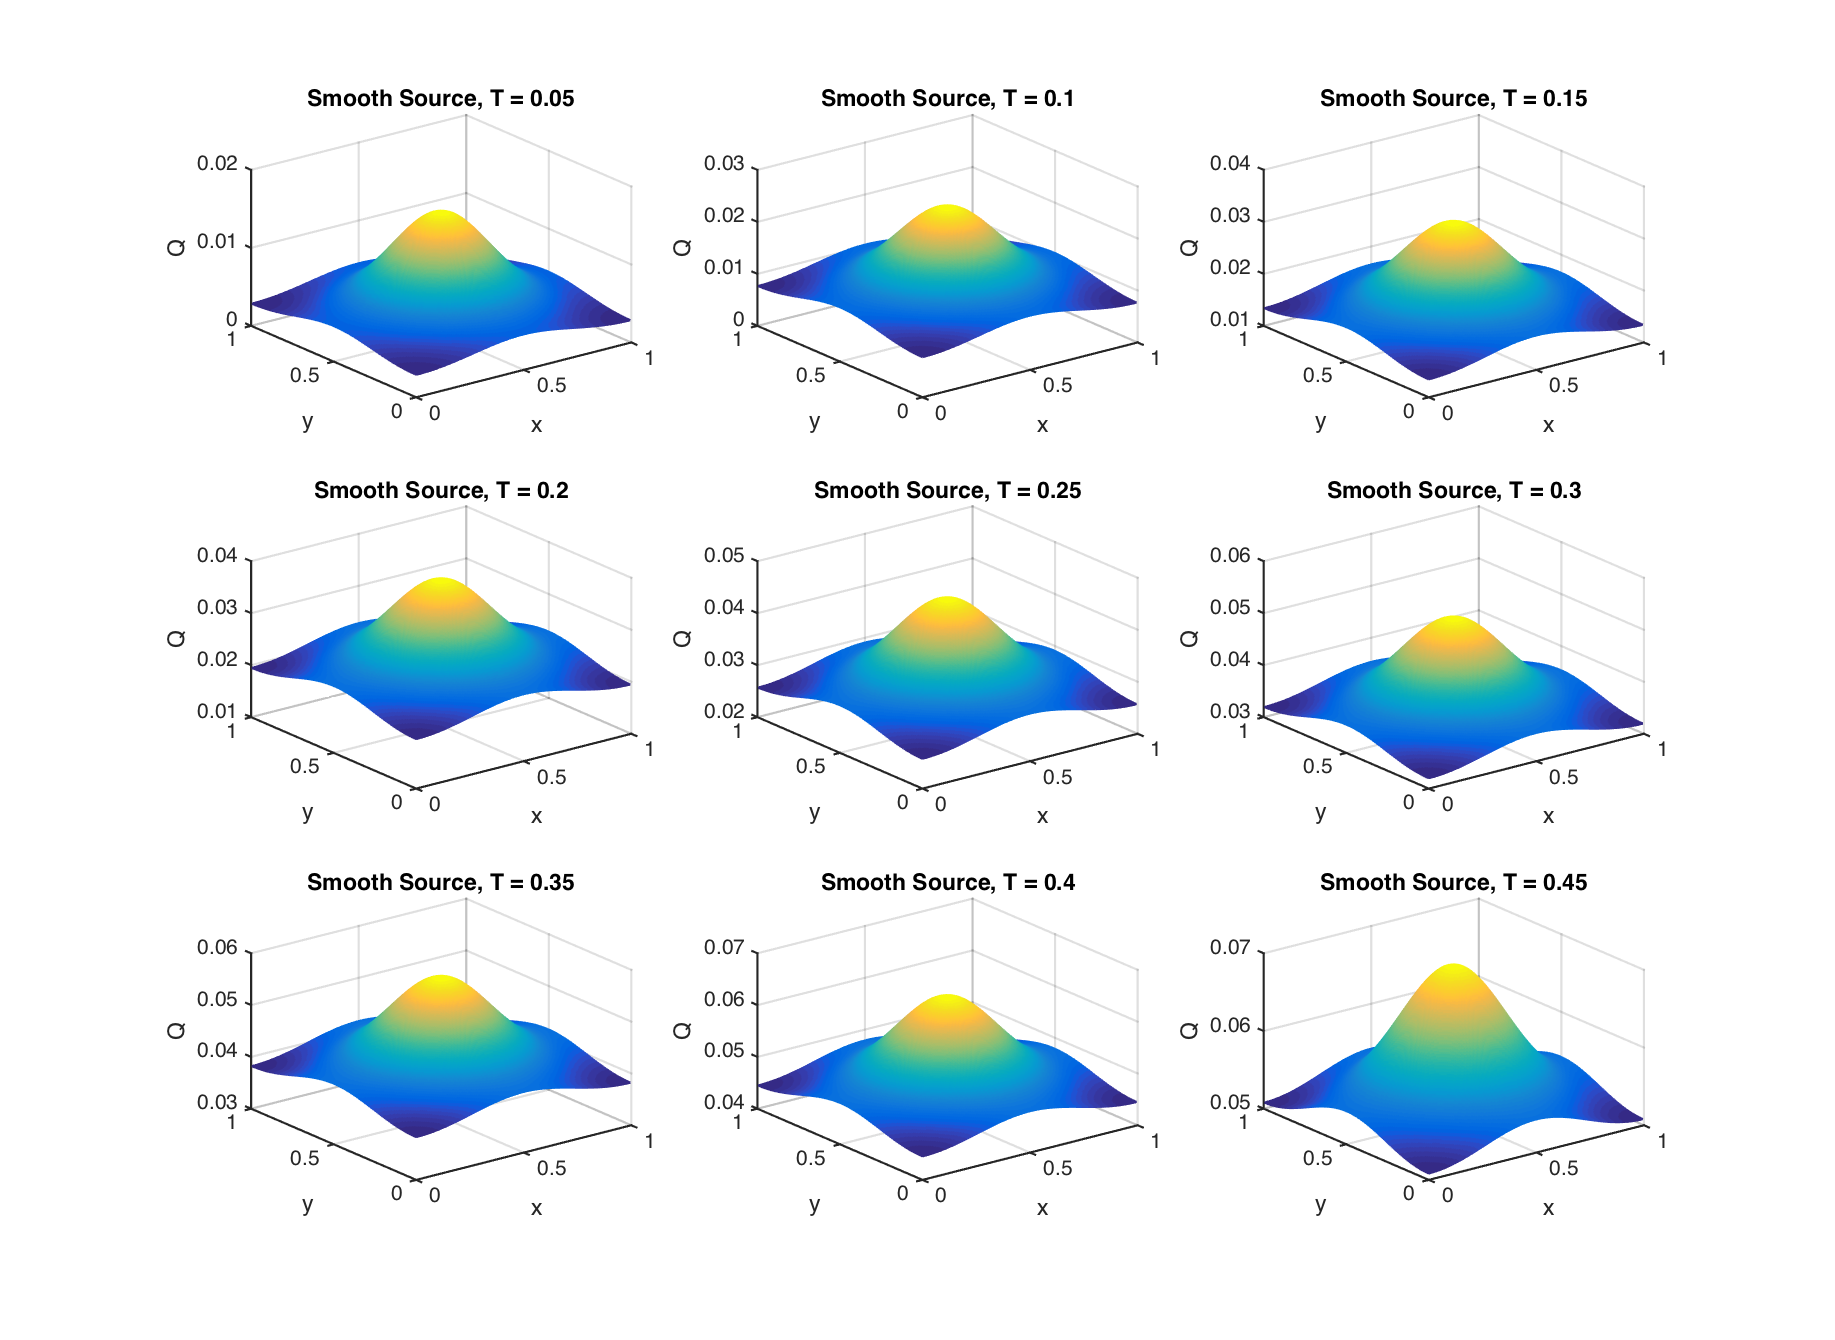
\includegraphics[scale=.5]{smoothSource4_1.eps}
\caption{Smooth Source Solutions at Different Times}
\label{fig:digraph}
\end{figure}
As we can see with the constant heat source, the total temperature is constantly increasing with the hottest part being at heat source.
\begin{figure}[!htb]
\centering
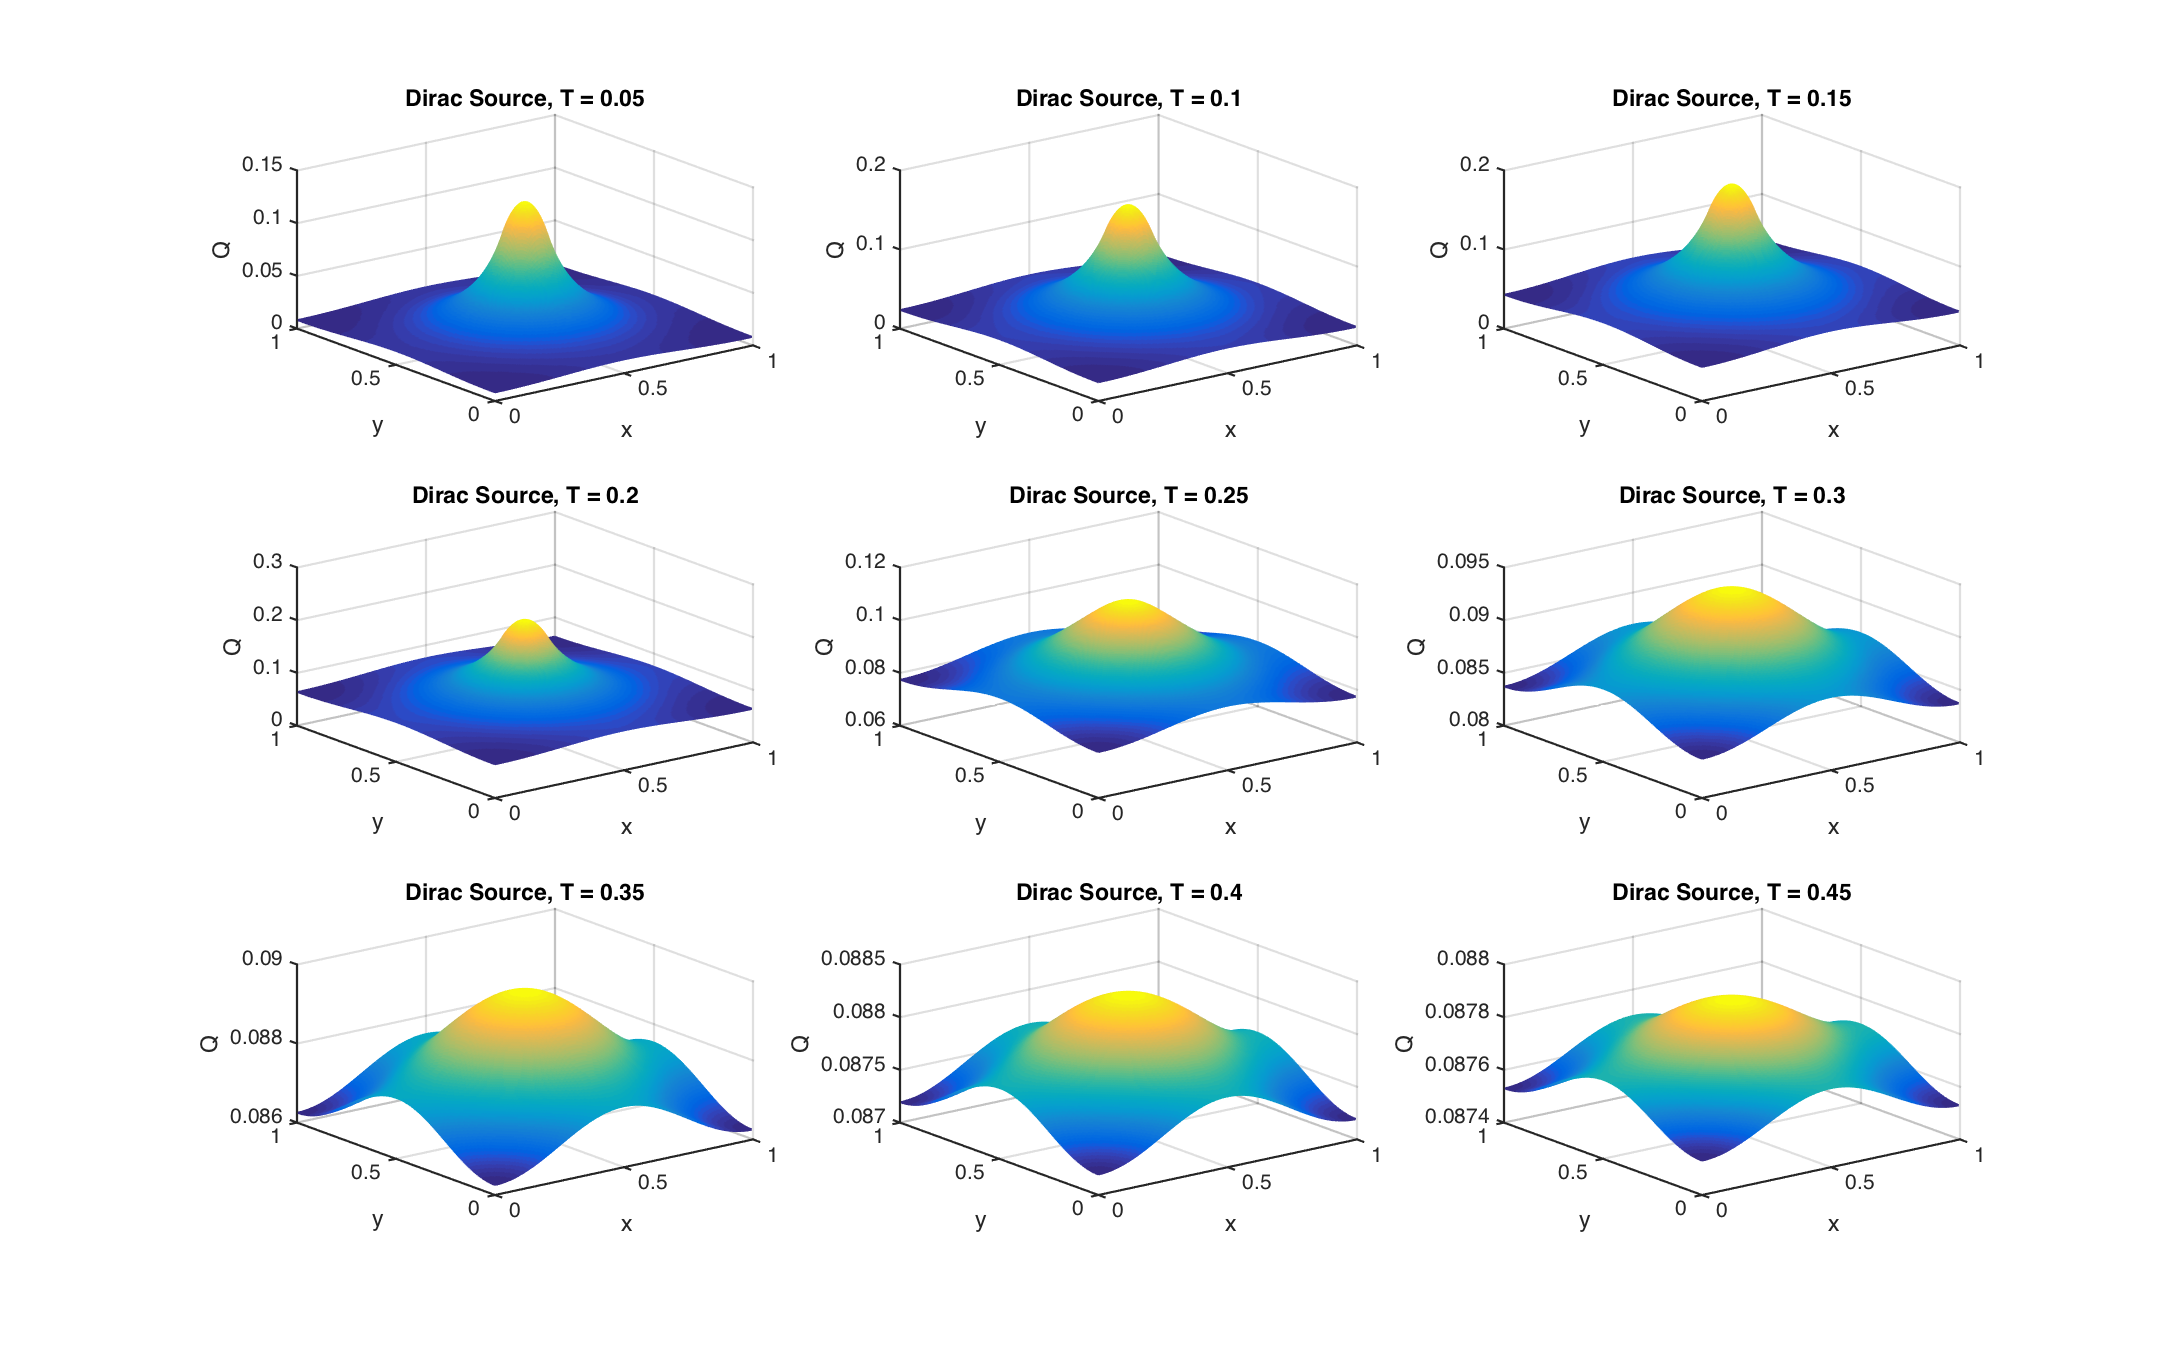
\includegraphics[scale=.5]{diracSource4_1.eps}
\caption{Dirac Source Solutions at Different Times}
\label{fig:digraph}
\end{figure}
Up until $T=0.25$, we observe the same phenomena that we observe for the smooth heat source. However, once we pass $T=0.25$, the total heat stays the same and starts to level out. 
\subsection{Convergence}
Because we do not know the true solution to the problem, we study ratios, which we denote by $R$, of the differences of the computed values i.e. 
\begin{align*}
R_h=\frac{Q'_{h/2,t} - Q'_{h,t}}{Q'_{h/4,t} - Q'_{h/2,t}}
\end{align*}
where, for example, $Q'_{h/2,t}$ is our computed solution using $\Delta x = \Delta y = h/2$ and $\Delta t = t$. We wish to show that the error behaves as $O(\Delta t^p) + O(\Delta h^r)$ and find $p$ and $r$. Letting $Q*$ denote the true solution, we write write our ratio as  
\begin{align*}
R_h = \frac{Q*+O(\Delta t^p) + O(\Delta (h/2)^r) - (Q* + O(\Delta t^p) + O(\Delta h^r))}{Q*+O(\Delta t^p) + O(\Delta (h/4)^r) - (Q*+O(\Delta t^p) + O(\Delta (h/2)^r))} = \frac{O(\Delta (h/2)^r)-O(\Delta h^r)}{O(\Delta (h/4)^r) - O(\Delta (h/2)^r)}
\end{align*}
To get the order of convergence from $R$, we take the log base 2. This gives us 
\begin{align*}
log_2(R_h) &= log_2(\frac{O(\Delta (h/2)^r)-O(\Delta h^r)}{O(\Delta (h/4)^r) - O(\Delta (h/2)^r)}) \\ 
&= log_2(\frac{2^{-r}O(\Delta h^r)-O(\Delta h^r)}{2^{-r}(2^{-r}O(\Delta h^r)-O(\Delta h^r))}) \\
&= log_2(2^{r}) \\
&= r
\end{align*}
We compute several values of $log_2(R_h)$ using different h values. We get the following values
\begin{table}[]
\centering
\caption{Order of Convergence in h}
\label{my-label}
\begin{tabular}{|c|c|c|c|}
\hline 
 & h=0.025 & h=0.0125 & 0.00625 \\ 
\hline 
$log_2(R)$ & 1.9962 & 1.9990 & 1.9986 \\ 
\hline 
\end{tabular} 
\end{table}
from which we can infer that $r = 2$. We do the same thing in $t$ with
\begin{align*}
R_t = \frac{O(\Delta (t/2)^p)-O(\Delta t^p)}{O(\Delta (t/4)^p) - O(\Delta (t/2)^p)}
\end{align*} 
and obtain the following values
\begin{table}[]
\centering
\caption{Order of Convergence in t}
\label{my-label}
\begin{tabular}{|c|c|c|c|}
\hline 
 & $t=4*10^{-4}$ & $t=2*10^{-4}$ & $t=1*10^{-4}$ \\ 
\hline 
$log_2(R_t)$ & 1.0000 & 1.0000 & 1.0000 \\ 
\hline 
\end{tabular} 
\end{table}
from which we infer that $p=1$. This values are in agreement with numerical theory because the derivative with respect to time is computed with the first order Euler scheme, which has first order convergence, and second order finite difference for the second derivative with respect to time, which has second order convergence. 

With the time variable source, we would expect the same $r$ and $p$, because we would use the same numerical methods. We obtain the same $p$ right away, although we do not obtain the same $r$ value. This is a result of the source term being dependent on $\Delta h$, and therefore changing with each of the different $\Delta h$ values we use. However, when solving for $r$ if we intervene in the program to keep the $\epsilon$ value the same for the different values of $h$, we can obtain the expected quadratic convergence in space. With a fixed $\epsilon =  \sqrt{\frac{1}{40}}$ we get $log_2(R_h) = 1.9978$ when $h=\frac{1}{160}$
Because the $\infty$ and $L^2$ norms are not defined, we do not look at them for the error. 
We now investigate the effect of refining our approximation of the Dirac function. We do this by changing $ \epsilon$ to $\alpha \sqrt{h}$ where $\alpha = 1,0.1,0.01,0.0001,$ and $10^{-10}$. 
We include the following plots with $\Delta h = 3.125*10^{-3}$ and $T=0.145$ show the effect of a more refined Dirac function. 
\begin{figure}[!htb]
\centering
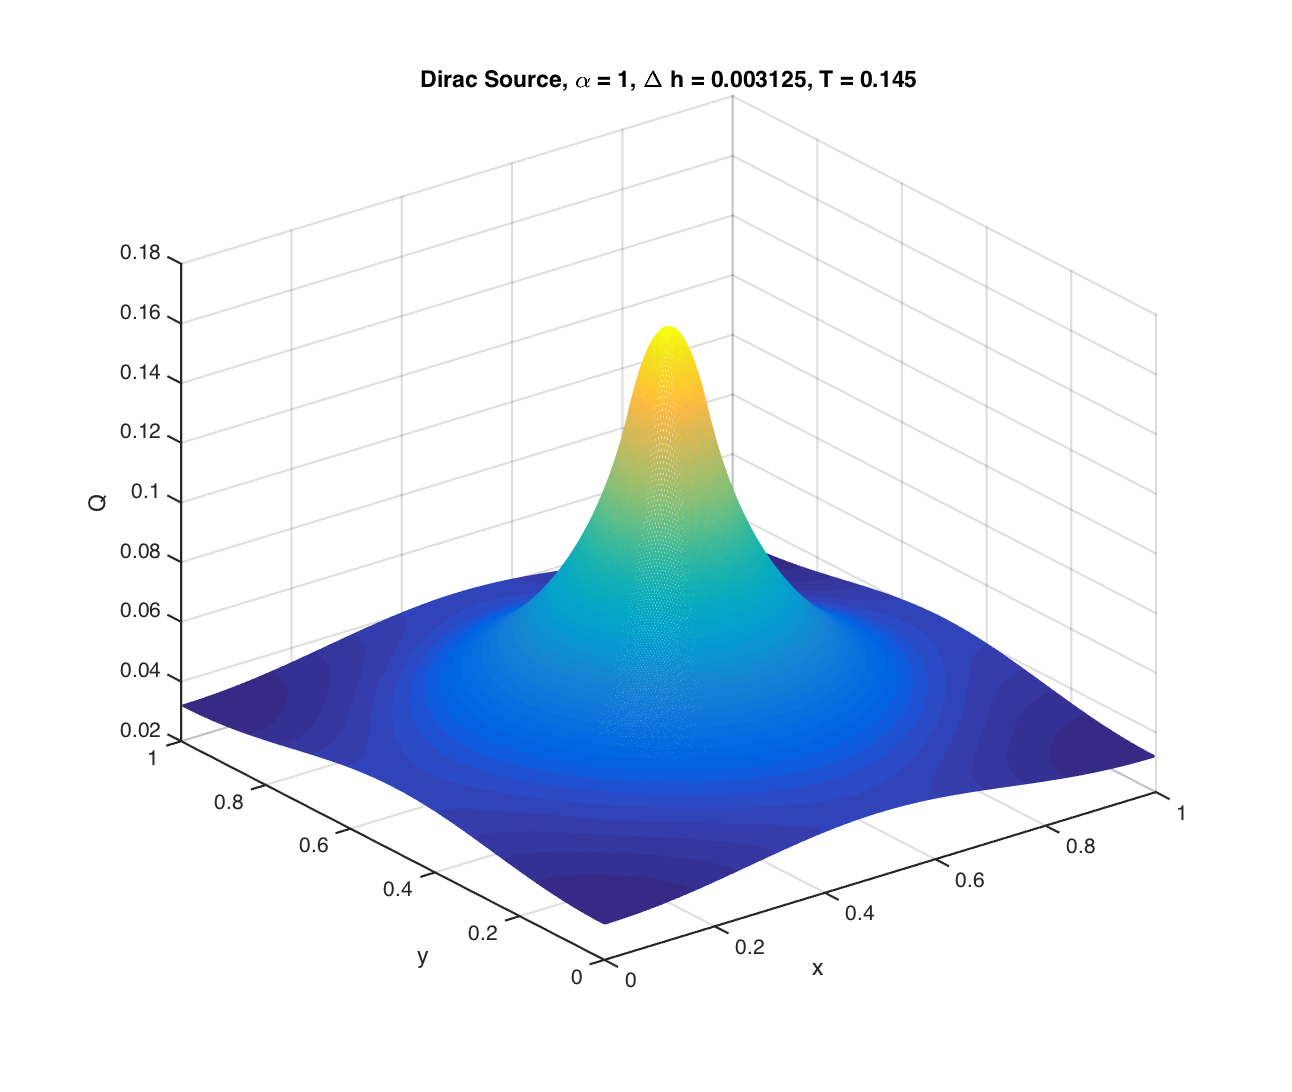
\includegraphics[scale=.6]{4_2_a_1.eps}
\caption{$\alpha = 1$}
\label{fig:digraph}
\end{figure}

\begin{figure}[!htb]
\centering
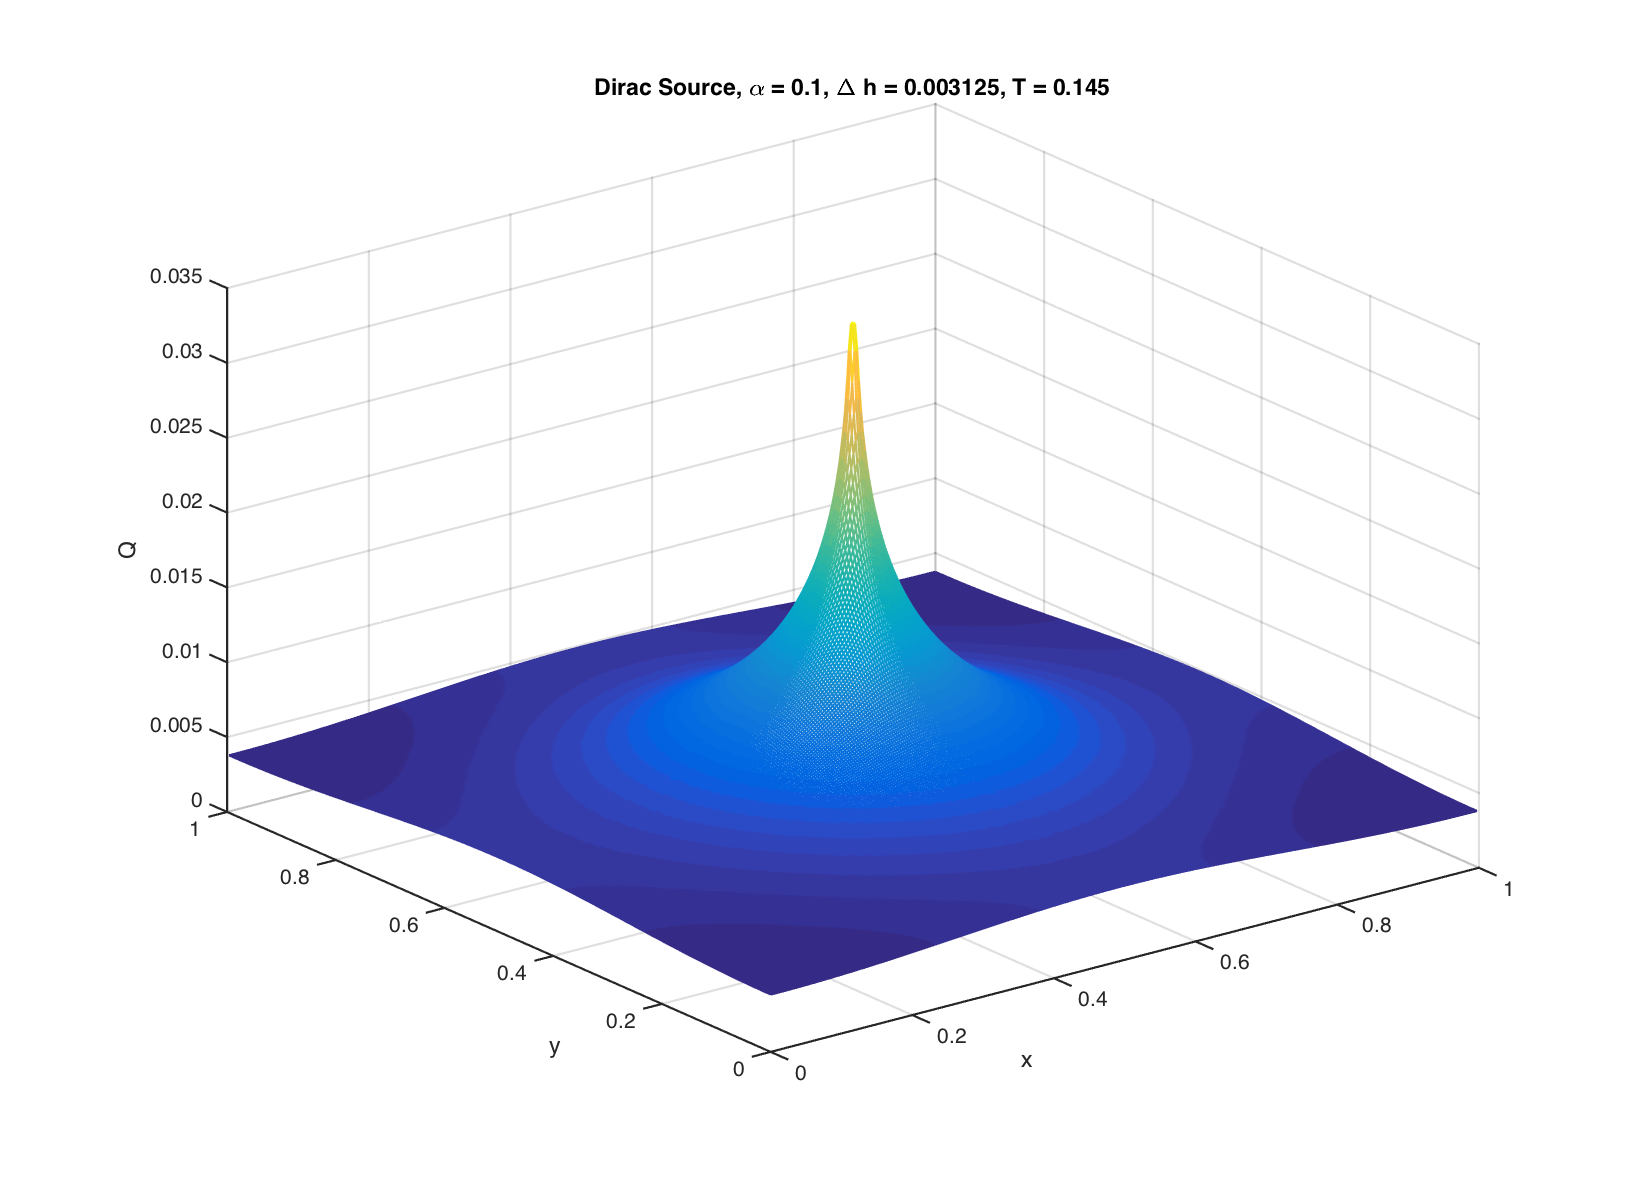
\includegraphics[scale=.6]{4_2_a_2.eps}
\caption{$\alpha = 0.1$}
\label{fig:digraph}
\end{figure}

As we can see, the peak becomes thinner and lower as $\alpha$ becomes smaller. We can see why this is when we look at the definition of the Dirac function. When $\alpha$ becomes smaller by a factor of 10, $\delta_{\epsilon}(r)$ increases by a factor of 10. But when doing this, we also cut down the accepted radius by a factor of 10. This radius defines an area that the heat source effects, which now has been but down by a factor of 100. This is why the peak becomes thinner and lower.

\subsection{Conservative}